
\chapter{بارسپاری کارآمد لبه شبکه برای نسل چهارم صنعت}\label{chap:model}

این فصل مدل سامانه‌ی جانمایی کانتینر و بارسپاری در طرح‌های \lr{\tt{MEC}} نسل چهارم صنعت را ارائه می‌دهد. مدل تحلیل کارایی آگاه از رقابت معرفی شده، مسئله‌ی بهینه‌سازی برای جانمایی کانتینر فرموله و پیکربندی شبیه‌سازی توضیح داده می‌شود. نتایج و تحلیل‌ها نیز برای نشان دادن امکان‌پذیری رویکرد پیشنهادی در این فصل قرار دارد.

\section{مدل پزدارش لبه شبکه در نسل چهارم صنعت}

محیط‌های مدرن نسل چهارم صنعت مانند کارخانه‌های هوشمند، انبارهای خودکار و سکوهای نفتی از تعداد زیادی دستگاه به‌هم‌پیوسته شامل ربات‌ها، وسایل نقلیه هدایت‌شونده خودکار، حسگرها و دوربین‌ها تشکیل شده‌اند. هر یک از این دستگاه‌های هوشمند قادر به حس کردن، برقراری ارتباط و در برخی موارد انجام محاسبات محلی هستند. کاربردهای صنعتی اغلب شامل وظایف عادی (مانند پایش دوره‌ای، ارسال سیگنال‌های کنترلی) و همچنین وظایف حساس به تأخیر (مانند تشخیص خطر توسط دوربین‌ها، جلوگیری از برخورد برای ربات‌ها یا بازرسی کیفی بلادرنگ در خطوط مونتاژ) می‌شوند.

اگرچه بسیاری از دستگاه‌ها به واحدهای پردازشی محلی مجهز هستند، اما اجرای صرفاً محلی در موارد متعددی کافی نیست:

\begin{itemize}
\item
\textbf{عدم رعایت کیفیت خدمت:} ممکن است یک دستگاه توان اجرای یک وظیفه حساس به تأخیر را در مهلت مقرر نداشته باشد، که این موضوع خطر بروز خطاهایی از کاهش جزئی بهره‌وری تا ایجاد مخاطرات جدی ایمنی را به همراه دارد.
\item
\textbf{بار بیش از حد ناشی از وظایف همزمان:} اگر یک ربات یا حسگر مشغول به یک وظیفه محلی باشد، ورود یک وظیفه جدید را ممکن است نتواند مدیریت کند. در این صورت نیازمند کمک از طرف یک پردازنده دیگر خواهد بود.
\item
\textbf{محدودیت‌های سخت‌افزاری:} برخی از دستگاه‌های اینترنت اشیا توان پردازشی قابل توجهی ندارند و فقط آماده ارسال داده مربوط به حسگرهای خود هستند تا پردازش در مکانی دیگر انجام شود.
\item
\textbf{محدودیت انرژی:} دستگاه‌های اینترنت اشیاء علاوه بر محدودیت پردازش، محدودیت مهم‌تر انرژی دارند. انرژی خود را از یک باتری محدود و ضعیف تامین میکنند و در صورتی که از پردازنده در این دستگاه‌ها استفاده شود موجب تخلیه باتری و خاموش شدن دستگاه می‌شود.
\end{itemize}

برای غلبه بر این محدودیت‌ها، برون‌سپاری وظایف ضروری می‌شود. با انتقال وظایف محاسباتی سنگین به سرورهای توانمندتر، دستگاه‌های صنعتی می‌توانند الزامات سخت‌گیرانه زمانی را برآورده کنند. در حالی که رایانش ابری به طور سنتی مقصد برون‌سپاری بوده است، پردازش مبتنی بر ابر به دلیل تأخیرهای ارتباطی گسترده، لغزش زمان پاسخگویی و ازدحام غیرقابل پیش‌بینی در اینترنت، با تأخیر بالا و غیرقابل پیش‌بینی روبه‌رو است. در نتیجه، زیرساخت‌های ابری نمی‌توانند زمان‌های پاسخ قطعی موردنیاز برای وظایف صنعتی حساس به تأخیر را تضمین کنند. برای رفع این محدودیت‌ها، پردازش لبه شبکه به عنوان یک راهکار عملی مطرح شده است. مطابق شکل~\ref{figure:system_model} سرورهای \lr{\tt{MEC}} در نزدیکی دستگاه‌های صنعتی مستقر می‌شوند و در حالی که ظرفیت پردازشی بیشتری نسبت به پردازنده دستگاه‌های محلی فراهم می‌کنند، تأخیر رفت و برگشت را به طور چشمگیری کاهش می‌دهند. با این حال، برون‌سپاری نیز چالش‌های جدیدی را به همراه دارد. تصمیم‌گیری در رابطه با برون‌سپاری پیچیدگی‌هایی دارد که به آن می‌پردازیم. برون‌سپاری نیازمند یک تصمیم‌گیری مرکزی‌ است. یک هماهنگ‌کننده متمرکز یا مدیر شبکه، فرآیند برون‌سپاری را کنترل می‌کند. این هماهنگ‌کننده آگاهی سراسری از وضعیت سامانه دارد، از جمله:

\begin{itemize}
\item
مکان‌های فیزیکی دستگاه‌های هوشمند و سرورهای \lr{\tt{MEC}}
\item
وضعیت ارتباطی دستگاه‌ها (نرخ‌های انتقال در ارتباط بالارونده/پایین‌رونده)
\item
بار پردازشی محلی روی پردازنده دستگاه‌ها
\item
میزان استفاده فعلی و در دسترس سرورهای \lr{\tt{MEC}}
\item
اطلاعات وظایفی که قبلاً برون‌سپاری شده‌اند
\end{itemize}

هنگامی که هر دستگاهی یک وظیفه جدید برای انجام دارد، اطلاعات و مشخصات این وظیفه را تحت عنوان یک درخواست برای مدیر شبکه ارسال می‌کند. این اطلاعات شامل اندازه داد‌های ورودی و خروجی وظیفه، تعداد چرخه‌های پردازنده برای اجرا،‌ مهلت زمانی، برنامه درخواست شده توسط وظیفه و حداقل میزان توان پردازشی مورد نیاز است. مدیر شبکه با اطلاعاتی که از وضع موجود شبکه داشت و اطلاعات درخواست‌های جدید باید تصمیم‌گیری مناسبی برای بارسپاری وظایف انجام دهد. این تصمیم‌گیری با هدف‌های مشخصی باید بهینه شود. هدف اول بیشینه کردن وظایف تخصیص‌یافته با رعایت محدودیت‌های سخت‌افزاری و مهلت وظایف است. هدف ثانویه بیشینه کردن حدفاصل بین تاخیر اجرای وظیفه با مهلت انجام آن است. این هدف باعث می‌شود حاشیه امن کافی برای اجرای یک وظیفه در نظر گرفته شود.

\vspace{0.5cm}
\begin{figure}[h]
\centering
\includegraphics[width=\textwidth]{system_model.pdf}
\caption{مدل سامانه مساله پردازش لبه شبکه در نسل چهارم صنعت.}
\label{figure:system_model}
\end{figure}
\vspace{0.5cm}

\subsection{کانتینرها در پردازش لبه شبکه}

یکی دیگر از عناصر مهم در مساله \lr{\tt{MEC}} پیشنهادی، کانتینری کردن برنامه‌هاست. برای اطمینان از استقرار سریع، زمان راه‌اندازی کوتاه و کاهش سربار در مقایسه با ماشین‌های مجازی، سرورهای \lr{\tt{MEC}} برنامه‌ها را درون کانتینرهای سبک‌وزن راه‌اندازی می‌کنند. هر کانتینر کتابخانه‌ها و وابستگی‌های موردنیاز برنامه مربوطه را در خود جای می‌دهد. یک کانتینر از یک لایه تصویر ایجاد می‌شود. در حالی که در محیط‌های \lr{\tt{MEC}} عمومی ممکن است لایه تصویر نیاز به بارگیری از مرکز داده را داشته باشند، در محیط صنعتی مجموعه برنامه‌های مورد نیاز از پیش شناخته شده است. بنابراین، سرورهای \lr{\tt{MEC}} لایه‌ تصویر کانتینر را ذخیره می‌کنند و تاخیر بارگیری آن را حذف کرده و اجرای فوری وظایف را ممکن می‌سازند.

\subsection{تاخیر مخابره و مصالحه پردازش و مخابره}

تأخیر ارتباطی یکی از اجزای مهم در تأخیر برون‌سپاری‌ است. پس از اتخاذ تصمیم برون‌سپاری برای یک وظیفه مشخص، تأخیر از مراحل مختلف در طول مسیر ارتباطی ناشی می‌شود. ابتدا، انتقال بالارونده از دستگاه صنعتی به نقطه دسترسی (\lr{\tt{AP}})\LTRfootnote{Access Point (AP)} متصل با آن، انجام می‌شود. تاخیر این ارسال به اندازه داده‌های ورودی وظیفه و نرخ انتقال بی‌سیم تخصیص‌یافته به دستگاه بستگی دارد. پس از رسیدن درخواست به \lr{\tt{AP}}، از طریق شبکه سیمی به سرور \lr{\tt{MEC}} هدف منتقل می‌شود. نرخ انتقال اتصال سیمی بین \lr{\tt{AP}} و سرور \lr{\tt{MEC}} تأخیر انتقال سیمی را تعیین می‌کند. پس از اتمام پردازش، داده‌های پاسخ باید به دستگاه مبدأ بازگردانده شوند. تأخیر پایین‌رونده بر اساس اندازه داده‌های خروجی و نرخ انتقال پایین‌رونده تخصیص‌یافته به دستگاه محاسبه می‌شود. بنابراین، تأخیر کلی ارتباطی برابر با جمع تأخیرهای بالارونده و پایین‌رونده در شبکه است.

تخصیص نرخ انتقال می‌تواند پیچیدگی متفاوتی داشته باشد. یک روش ساده، تخصیص یکنواخت است، که در آن \lr{\tt{AP}} پهنای باند را به طور مساوری بین تمام دستگاه‌های متصل صرف‌نظر از توان انتقال یا کیفیت کانال آن‌ها، ارائه می‌دهد. اگرچه این روش ساده است، ممکن است بهره‌وری را بیشینه نکند. اگرچه راهبردهای تخصیص پیشرفته‌تر می‌توانند برای بهینه‌سازی تأخیر و انصاف در نظر گرفته شوند، اما فرض تخصیص یکنواخت یک پایه قابل استفاده برای تخمین تأخیرهای ارتباطی را فراهم می‌کند.

تأخیر ارتباطی مصالحه‌ای پر تکرار در مقالات، برای تصمیم‌گیری برون‌سپاری در مقابل قدرت بیشتر پردازش مرکزی است. در حالی که برون‌سپاری وظایف به سرورهای \lr{\tt{MEC}} دسترسی به توان پردازشی بالاتر را فراهم می‌کند و ممکن است تأخیرهای پردازش محلی را کاهش دهد، هم‌زمان تأخیر اضافی ناشی از انتقال ‌داده‌های وظیفه را ایجاد می‌کند. بنابراین، تصمیم برون‌سپاری نمی‌تواند تنها بر اساس توان محاسباتی سرور \lr{\tt{MEC}} گرفته شود؛ بلکه باید مزایای پردازش سریع‌تر را در مقابل جریمه‌ تأخیر ارتباطی به دقت سبک سنگین کرد. برای وظایف حساس به تأخیر، اگر مجموع تأخیرهای پردازشی و مخابره از مهلت زمانی درخواست فراتر رود، برون‌سپاری نتیجه معکوس می‌دهد و اجرای محلی علی‌رغم کندتر بودن پردازش، ترجیح داده می‌شود. برعکس، برای وظایفی با نیازهای محاسباتی زیاد اما اندازه داده‌ی متوسط، برون‌سپاری می‌تواند به کاهش تاخیر منجر شود.

\section{تداخل برنامه‌ها}
\label{subsec:interference_model}

فراتر از ارتباط با نقاط دسترسی، محیط مشترک دیگر، منابع سخت‌افزاری سرورهای \lr{\tt{MEC}} هستند که زمینه تداخل ایجاد می‌شود. هنگامی که چندین کانتینر روی یک سرور مشترک مستقر می‌شوند، ناگزیر برای منابع مشترک رقابت می‌کنند که این موضوع می‌تواند منجر به افت عملکرد شود. اگرچه مجازی‌سازی تا حدی جداسازی ایجاد می‌کند، اما همه منابع سخت‌افزاری قابل جداسازی کامل نیستند. حافظه‌نهان‌، پهنای‌باند حافظه، ورودی/خروجی فضای ذخیره‌سازی و واسط‌های شبکه همچنان نقاط بروز رقابت محسوب می‌شوند. در نتیجه، دومین مصالحه مهم در تصمیم‌گیری برون‌سپاری شکل می‌گیرد: هرچند سرورهای \lr{\tt{MEC}} توان پردازشی بالاتری نسبت به دستگاه‌های محلی ارائه می‌دهند، عملکرد آن‌ها در شرایط تداخل شدید ممکن است کاهش یابد و گاهی مزایای حاصل از برون‌سپاری را خنثی کند.

یکی از راه‌های کاهش تداخل، استفاده از سیاست‌های زمان‌بندی است. برنامه‌ها الگوهای متفاوتی از خود نشان می‌دهند، مانند محاسبه‌محور، حافظه‌محور، ورودی/خروجی ‌محور برای فضای ذخیره‌سازی و شبکه. در حالت ایده‌آل، برنامه‌های مکمل باید در کنار یکدیگر زمان‌بندی شوند، در حالی که برنامه‌هایی که بر یک منبع مشابه فشار وارد می‌کنند باید از هم جدا شوند. به این قائده هم‌پیوندی گفته می‌شود. با این حال، پردازش لبه شبکه با تعداد کم سرورهای \lr{\tt{MEC}} و محدودیت منابع سرورها، پایبندی به قوانین هم‌پیوندی همیشه عملی نیست. حتی در صورت هم‌مکانی برنامه‌هایی با الگوهای مشابه، عدم امکان پاسخگویی در مهلت مقرر قطعی نیست، ممکن است رخ دهد یا ندهد. بنابراین، بدون پیش‌بینی کمّی اثرات تداخل، اتخاذ تصمیمات قابل اعتماد در زمینه برون‌سپاری و زمان‌بندی دشوار می‌شود.

پژوهش ما با معرفی یک مدل کمّی از تداخل چندین برنامه، خود را از کارهای پیشین متمایز می‌کند. مطالعات موجود، مانند مدل تداخل ارائه‌شده در \cite{medel2023modeling}، چارچوبی برای تخمین در مورد دو برنامه که همزمان اجرا می‌شوند فراهم می‌آورند. رویکرد آن‌ها شامل جمع‌آوری آمارهای سطح پایین عملکرد (مانند چرخه‌های پردازنده، دستورالعمل‌های اجراشده، برخوردها و خطاهای حافظه‌نهان، و خطاهای صفحه\LTRfootnote{Page faults}) از برنامه‌هایی است که به صورت تنها اجرا می‌شوند. سپس با تبدیل آمار سطح پایین به چهار عامل مستقل: میزان استفاده از پردازنده، خطاهای صفحه حافظه، شدت سلسله‌مراتب حافظه و شدت استفاده از حافظه‌نهان توصیف تداخل را انجام می‌دهند. سپس مدل، تداخل دو برنامه هم‌مکان‌شده را با استفاده از فرمول‌بندی~\eqref{eq:medel_contention} تخمین می‌زند.

\begin{equation} \label{eq:medel_contention}
    C_{a_1 \otimes a_2} = \beta_0 + \sum_n^4 \beta_n P_n + \sum_n^4 \beta_{n+4}P'_n
\end{equation}

در اینجا، $C$ نشان‌دهنده ضریب تداخلی است که برنامه $a_2$ بر برنامه $a_1$ تحمیل می‌کند و نشان‌دهنده میزان افت کیفیت اجراست. عملگر نامتقارن $\otimes$ تداخل را نمایش می‌دهد. ضرایب $b_n$ با استفاده از تحلیل رگرسیون و بر اساس کاربارهای محک به‌دست می‌آیند (\lr{\tt{POV-Ray}} فشار بر پردازنده، \lr{\tt{STREAM}} فشار بر پهنای‌باند حافظه و \lr{\tt{IOZone}} فشار ورودی/خروجی). این برنامه‌های محک گلوگاه‌های خاص منابع را برای تخمین مدل تداخل برجسته می‌سازند و حساسیت برنامه به تداخل در منبع مشخصی را نمایان می‌سازند. پس از به‌دست‌آوردن ضرایب، با داشتن مدل یک برنامه، تداخل را می‌توان تنها با اندازه‌گیری عوامل برنامه مداخله‌گر در حالت ایزوله پیش‌بینی کرد.

این رویکرد دو مزیت کلیدی ارائه می‌دهد:

\begin{itemize}
\item
\textbf{مقیاس‌پذیری:} نیازی به اندازه‌گیری جامع تمام ترکیب‌های ممکن برنامه‌ها وجود ندارد. اجرای ایزوله همراه با آزمون‌های محک برای ساخت مدل‌های پیش‌بین کافی است.
\item
\textbf{قابلیت تفسیر:} تداخل با عوامل قابل‌درک برای انسان توصیف شده و مستقیماً با الگوهای استفاده از منابع مطابقت دارند. عوامل توصیف کننده تداخل، مانند یک آمار سطح پایین (برای مثال تعداد چرخه‌های پردازنده) نیستند که نتوان از خوانش آن به تفسیری در مورد بهره‌وری منابع رسید. از طرفی پس از تبدیل‌های ریاضی لگاریتمی و خطی همچنان به قدر کافی تفسیر پذیر هستند که یک معیار پیچیده و غیرقابل فهم نشده باشند.
\end{itemize}

با این حال، یک محدودیت اساسی همچنان باقی می‌ماند: این مدل برای ثبت رفتار بیش از دو برنامه که به طور همزمان هم‌مکان می‌شوند طراحی نشده است. برای ارزیابی برنامه‌های تداخلگر، جمع ساده عوامل مانند رابطه~\eqref{eq:false_interference_model} (عوامل $P_n”$ برای برنامه سوم است)نمی‌تواند پویایی واقعی رقابت چندبرنامه‌ای را بازتاب دهد زیرا برنامه‌های تداخلگر هم موجب افت کارایی یکدیگر شده و این رابطه تنها به ایجاد تداخل هر برنامه بر برنامه مورد نظر می‌پردازد.

\begin{equation} \label{eq:false_interference_model}
    C_{a_1 \otimes (a_2, a_3)} = \beta_0 + \sum_n^4 \beta_n P_n + \sum_n^4 \beta_{n+4}(P'_n + p"_n)
\end{equation}

از طرفی نمی‌توان یک مدل با ضرایب متمایز برای برنامه‌های سوم و بیشتر مانند رابطه~\eqref{eq:false_interference_model2} ارائه کرد. زیرا با ورود ضرایب فاکتور‌های برنامه سوم و باقی برنامه‌ها برای بدست آوردن ضرایب باید ترکیب‌های زیادی از برنامه مورد نظر را با برنامه‌های محک اجرا کرد. بنابراین مقیاس‌پذیری اندازه‌گیری‌ها و تخمین را از بین می‌برد.

\begin{equation} \label{eq:false_interference_model2}
    C_{a_1 \otimes (a_2, a_3)} = \beta_0 + \sum_n^4 \beta_n P_n + \sum_n^4 \beta_{n+4}P'_n + \sum_n^4 beta_{n+8}P"_n + ...
\end{equation}

در این رساله، ما فرمول‌بندی دوبرنامه‌ای را به یک مدل تعمیم‌یافته تداخل برای طرح‌های چندبرنامه‌ای در \lr{\tt{MEC}} گسترش می‌دهیم تا پیش‌بینی دقیق عملکرد و تخصیص منابع برای وظایف حساس به تأخیر نسل چهارم صنعت را ممکن سازیم. برای محاسبه تداخل بین چند برنامه از ایده برنامه مرکب استفاده می‌کنیم. یعنی تداخل دو تداخلگر بر برنامه مورد نظر ما، با یک برنامه مرکب مدل شده و عوامل برنامه مرکب را در رابطه مطرح شده ~\eqref{eq:medel_contention} استفاده می‌کنیم.

رابطه~\eqref{eq:compound_app} نشانگر نحوه محاسبه فاکتور‌های تداخلی برنامه مرکب شامل دو برنامه است. در این رابطه برنامه مرکب شامل $\{a_2, a_3\}$ است. هر عامل برنامه مرکب با ضرب همان عامل برای برنامه‌ها در تداخل ناشی از برنامه دیگری است. $C_{a_2 \otimes a_3}$ تداخل ناشی از $a_3$ بر $a_2$ و $C_{a_3 \otimes a_2}$ تداخل ناشی از $a_2$ بر $a_3$ است. به این ترتیب محاسبه عوامل برنامه مرکب به صورت متقارن انجام می‌گیرد. 

\begin{equation} \label{eq:compound_app}
    C_{a_2 \otimes a_3} \sum_n^4 P'_n + C_{a_3 \otimes a_2} \sum_n^4 P"_n
\end{equation}

این رابطه قابل تعمیم به هر تعداد برنامه است و هم‌چنین دارای مزایای زیادی است. 

\begin{enumerate}
\item
یکی از مزایای اصلی رویکرد تخمین تداخل معرفی‌شده در \cite{medel2023modeling} مقیاس‌پذیری است. ما با حفظ مقیاس‌پذیری در رابطه از ویژگی‌های برجسته مقاله مراقبت کردیم. این مدل نیازی به اندازه‌گیری جامع تمام ترکیب‌های برنامه‌ها ندارد. بلکه بر شاخص‌های عملکرد تنها و همراه برنامه‌های محک تکیه می‌کند. این ویژگی آن را در محیط‌های \lr{\tt{MEC}} و نسل چهارم صنعت بسیار کاربردی می‌سازد، جایی که تعداد برنامه‌ها و طرح‌های هم‌مکانی به‌صورت نمایی رشد می‌کند.
\item
مزیت دوم در توجیه فیزیکی مدل نهفته است. با ضرب‌کردن تداخل در عوامل بهره‌وری منابع، مدل اثرات واقعی سخت‌افزاری را بازتاب می‌دهد.

\begin{itemize}
\item
\textbf{عامل استفاده از پردازنده:} با ضرب در تداخل، نشان می‌دهد برنامه برای اجرا در مدت زمان قبلی نیازمند توان پردازشی بیشتری است که معادل تاثیر هم‌مکانی با تداخلگر است.
\item
\textbf{عامل خطای صفحه:} رقابت بیشتر بر سر حافظه، موجب افزایش نرخ خطای صفحه شده و ممکن است وابستگی به فضای \lr{\tt{swap}} را به دنبال داشته باشد. ضرب تداخل، کاملا نشان‌دهنده افزایش میزان خطای صفحه ناشی از هم‌مکانی با تداخلگر است.
\item
\textbf{عامل شدت استفاده از حافظه:} هنگامی که تداخل باعث افت کارایی می‌شود، پهنای‌باند حافظه به یک گلوگاه تبدیل می‌گردد. پردازش‌ها متوقف می‌شوند و عملیات بارگذاری/ذخیره‌سازی در چرخه‌های اضافی بسیاری ادامه می‌یابد، که این موضوع در عامل شدت استفاده از حافظه بازتاب پیدا می‌کند.
\item
\textbf{عامل شدت نرخ خطای حافظه‌نهان:} تداخل موجب نرخ خطای بیشتر حافظه‌نهان است و ضرب تداخل در عامل شدت نرخ خطای حافظه نهان با مفهوم فیزیکی معادل است.
\end{itemize}

\item
در نهایت، تخمین دست بالای تداخل توسط این رویکرد مدل‌سازی ارائه می‌شود. با ضرب تداخل در تمام عوامل، مدل یک حد بالای محافظه‌کارانه برای میزان افت کارایی ارائه می‌دهد. در عمل، همه عوامل به یک اندازه تحت تأثیر تداخل قرار نمی‌گیرند و برخی ممکن است نزدیک به مقادیر اجرای تنهای خود باقی بمانند. با این حال، این مدل تداخل با تخمین دست بالا، تضمین می‌کند که مدل برای برنامه‌های حساس به تأخیر، ایمن و قابل اعتماد باقی بماند، جایی که تخمین کم تداخل می‌تواند منجر به از دست رفتن مهلت‌های زمانی یا عدم توانایی پاسخگویی بشود.
\end{enumerate}

برای محاسبه تداخل بین برنامه‌ها، ضروری است که بدانیم کدام کانتینرها روی یک سرور هم‌مکان هستند. برای مثال برنامه‌های کانتینری در شکل راست \ref{figure:containers_combination} به نمایش درآمده است. در شکل راست همه ظرفیت سرور اختصاص یافته است. اما در شکل سمت چپ ترکیب متفاوتی از برنامه‌ها با دو جای خالی دیده می‌شود. همان‌طور که در این بخش بحث شد، تداخل با استفاده از روش برنامه مرکب مدل‌سازی می‌شود، به‌طوری که عوامل توصیف تداخل یک برنامه مرکب با ضرب عوامل هر برنامه به‌صورت جداگانه در میزان تداخل همه برنامه‌های داخل برنامه مرکب محاسبه می‌شود. فرض کنید یک سرور بتواند حداکثر $M$ کانتینر را میزبانی کند و $A$ برنامه متمایز برای استقرار وجود داشته باشد. تعداد کانتینرها روی یک سرور می‌تواند کمتر از ظرفیت بیشینه $M$ باشد. تمام ترکیب‌های ممکن استقرار را می‌توان با استفاده از انتخاب $\binom{M+A+1}{M}$ بدست آورد. در این عبارت پیکربندی‌هایی که در آن بخشی از ظرفیت سرور پر شده یا حتی خالی است نیز در نظر گرفته شده است. به‌عنوان مثال، فرض کنید $A=4$ برنامه و ظرفیت سرور $M=6$ کانتینر باشد. با استفاده از فرمول ترکیبیاتی، تعداد ترکیب‌های ممکن کانتینرها برابر است با $\binom{11}{6}=462$، که تمام الگوهای معتبر هم‌مکانی را در بر می‌گیرد. اهمیت آماده‌سازی همه ترکیب‌های ممکن پیش از فرمول‌بندی مساله بهینه‌سازی، مربوط به متغیر تصمیم‌گیری چیدمان کانتینرهای سرورها است.

\vspace{0.5cm}
\begin{figure}[h]
\begin{minipage}{0.45\textwidth}
\centering
\includegraphics[width=\textwidth]{containers_combination2.pdf}
\end{minipage}\hfill
\begin{minipage}{0.45\textwidth}
\centering
\includegraphics[width=\textwidth]{containers_combination.pdf}
\end{minipage}\hfill
\caption{چیدمان کانتینرها در سرور.}
\label{figure:containers_combination}
\end{figure}
\vspace{0.5cm}

\section{فرمول‌بندی مساله بهینه‌سازی}

در این بخش فرمول‌بندی مساله بهینه‌سازی ارائه می‌شود که توسط مدیر شبکه اجرا می‌شود و تصمیم‌گیری‌های لازم جهت بارسپاری را انجام می‌دهد. مطابق شکل~\ref{figure:system_model} دستگاه‌های هوشمند موجود در محیط صنعتی با $e$ نشان داده می‌شوند. هر دستگاه توان پردازشی محلی $F_e$ دارد و وظایفی تولید می‌کند که تحت عنوان درخواست‌های دستگاه $\mathbb{K}_e$ برای مدیر شبکه ارسال می‌شود. نرخ ارسال و دریافت نقطه دسترسی با دستگاه به صورت بی‌سیم، $R_{w,e,s}$ است. نرخ انتقال بین نقطه دسترسی و سرور $s$ نیز $R_{f,s}$ است. توان پردازشی سرور برابر با $F_s$ است. هر وظیفه در یک کانتینر قرار گرفته و در سرور اجرا می‌شود. اطلاعات هر درخواست $k$ شامل ابعاد داده ورودی $I_k$، ابعاد پاسخ خروجی $O_k$، مهلت پاسخگویی $\Theta_k$، چرخه‌های پردازنده لازم برای اجرای برنامه $L_k$، توان پردازشی مورد نیاز برای کانتینر مربوط $f^{con}_k$  و برنامه فراخوانی شده $a(k)$ است. برنامه‌های کانتینری موجود در سرور دارای یک چیدمان بدون ترتیب هستند که با اندیس $m$ و مجموعه برنامه‌ها با $\mathbb{A}_m$ نمایش داده می‌شوند. تداخل ایجاد شده روی برنامه فراخوانی شده توسط وظیفه $k$، با $C_{k,\mathbb{A}_m}$ نمیاش داده می‌شود. علائم استفاده شده در این پژوهش به طور خلاصه در جدول~\ref{table:problem_notations} آورده شده است.

\begin{table*}[h!]
\begin{center}
\caption{اندیس و مجموعه‌ها، مقادیر ثابت و متغیرهای مسئله بهینه‌سازی.}
\begin{tabular}{ |c|c|r|r| }
\hline
نوع & نماد & توضیح & مقدار \\ 
\hline
\multirow{10}{*}{\rotatebox[origin=r]{90}{مجموعه‌ها}} 
& $n$ & اندیس‌ عوامل تداخل & $\{0, 1, \dots, 8\}$ \\
& $e \in \mathbb{E}$ & مجموعه دستگاه‌ها (ربات‌ها و حسگرها) & $\{1, 2, \dots, |E|\}$ \\
& $s \in \mathbb{S}$ & مجموعه سرورهای \lr{\tt{MEC}} & $\{1, 2, \dots, |S|\}$ \\
& $a \in \mathbb{A}$ & مجموعه برنامه‌های & $\{1, 2, \dots, |A|\}$ \\
& $k \in \mathbb{K}$ & مجموعه‌ درخواست‌ها/وظایف & $\{1, 2, \dots, |K|\}$ \\
& $\mathbb{K}_e$ & وظایف دستگاه $e$ & مثلا $\{3, 4, \dots \}$ \\
& $\mathbb{K}_s$ & وظایف بارسپاری شده در $s$ & مثلا $\{3, 4, \dots \}$ \\
& $a(k)$ & برنامه وظیفه $k$ & \\
& $m \in \mathbb{M}$ & ترکیب‌های بدون ترتیب ممکن در سرور & \\
& $\mathbb{A}_m$ & برنامه‌های ترکیب $m$ & مثلا $(a_1,a_3, ..., |\mathbb{A}_m|)$ \\
\hline
\multirow{13}{*}{\rotatebox[origin=c]{90}{مقادیر ثابت}}
& $\mathcal{M}$ & بیشترین تعداد کانتینر بر روی سرور & \\
& $\beta_{a(k)}$ & بردار ضرایب تداخل برای یک برنامه & \\
& $P_{a(k)}$ & عوامل تداخل برای برنامه وظیفه $k$ & \\
& $I_k$ & ابعاد داده ورودی برای $k$ & $10$ مگابایت \\
& $O_k$ & ابعاد داده خروجی برای $k$ & $500$ کیلوبایت \\
& $L_k$ & چرخه‌های پردازنده لازم برای $k$ & $1000$ میلیون چرخه \\
& $\Theta_k$ & مهلت اجرای $k$ & $10$ ثانیه \\
& $F_s$ & توان پردازشی $s$ & $3$ گیگاهرتز \\
& $F_e$ & توان پردازشی محلی $e$ & $100$ مگاهرتز \\
& $f_k$ & توان پردازشی تخصیص یافته به کانتینر $k$ & $500$ مگاهرتز \\
& $R_{w,e,s}$ & نرخ ارسال بی‌سیم بین $e$ و نقطه دسترسی سرور $s$ & $50$ مگابیت بر ثانیه \\
& $R_{f,s}$ & نرخ ارسال سیمی بین نقطه دسترسی و سرور $s$ & $100$ مگابیت بر ثانیه \\
& $C_{k,\mathbb{A}_m}$ & تداخل ترکیب $m$ برای $k$ & \\
\hline
\multirow{3}{*}{\rotatebox[origin=c]{90}{متغیرها}} 
& $x_{k,e,s}$ & 1 اگر $k$ از $e$ به $s$ بارسپاری شود وگرنه 0 & \\
& $x_{k,e,0}$ & 1 اگر $k$ پردازش محلی در $e$ شود وگرنه 0 & \\
& $z_{s,m}$ & 1 اگر $s$ دارای ترکیب $m$ باشد وگرنه 0 & \\
\hline
\end{tabular}
\label{table:problem_notations}
\end{center}
\end{table*}

\subsection{فرمول پیشنهادی تداخل منابع}

همانطور که در بخش~\ref{subsec:interference_model} بحث شد، تداخل بین دو کانتینر بر اساس فرمول تداخل معرفی شده در مقاله \cite{medel2023modeling} در رابطه~\eqref{eq:mutual_interference} آمده است. بر این اساس تداخل بین دو برنامه $a_1$ که توسط وظیفه $k$ و $a_2$ که توسط وظیفه $k'$ فراخوانی شده محاسبه می‌شود. ترکیب $\mathbb{A}_m=\{a_1,a_2\}$ برنامه‌های سرور $s$ هستند و ضرایب $\beta_{a,n}$ در عامل‌های تداخل $P_{a,n}$ توصیف کننده تداخل $C_{k,\mathbb{A}_m}$ هستند.
\begin{equation} \label{eq:mutual_interference}
    C_{k,\mathbb{A}_m} = \beta_{a_1,0} + \sum_{n=1}^4 \beta_{a_1,n} P_{a_1,n} + \sum_{n=1}^4 \beta_{a_1,n+4} P_{a_2,n}
\end{equation}
گسترش این رابطه در این پژوهش با استفاده از ارائه مفهوم برنامه مرکب و تاثیردهی تداخل در عوامل هرکدام از اعضای برنامه مرکب است. بر این اساس اگر بخواهیم تداخل ترکیب سه برنامه را بررسی کنیم، رابطه~\eqref{eq:triple_interference} را معرفی می‌کنیم. در این رابطه برنامه $a_3$ توسط وظیفه $k"$ فراخوانی شده است. ترکیب برنامه‌ها $\mathbb{A}_m=\{a_1,a_2,a_3\}$ است. برای محاسبه تداخل در برنامه مرکب، ترکیب برنامه‌های برنامه مرکب در زیرمجموعه $\mathbb{A}'_m=\{a_2,a_3\}$ معرفی شده است. (برنامه $a_1$ که فرمول محاسبه تداخل برای آن نوشته می‌شود،نسبت به مجموعه $\mathbb{A}_m$ حذف شده)
\begin{equation} \label{eq:triple_interference}
    C_{k,\mathbb{A}_m} = \beta_{a_1,0} + \sum_{n=1}^4 \beta_{a_1,n} P_{a_1,n} + \sum_{n=1}^4 \beta_{a_1,n+4} \left(P_{a_2,n}C_{k',\mathbb{A}'_m} + P_{a_3,n}C_{k",\mathbb{A}'_m}\right)
\end{equation}
برای جمع‌بندی محاسبه تداخل برای برنامه‌ی وظیفه $a(k)$ در رابطه\eqref{eq:total_interference} آمده است. بر این اساس در برنامه مرکب، تداخل‌های پیش‌امده توسط دیگر برنامه‌ها در عامل‌های توصیف تداخل ضرب شده است.
\begin{equation} \label{eq:total_interference}
    C_{k,\mathbb{A}_m} = \beta_{a(k),0} + \sum_{n=1}^4 \beta_{a(k),n} P_{a(k),n} + \sum_{n=1}^4 \beta_{a(k),n+4} \left(\sum_{j \in \mathbb{K}_s} P_{a(j),n} C_{j,\mathbb{A}'_m}\right)
\end{equation}
رابطه~\eqref{eq:total_interference} که به صورت تکرار شونده به محاسبه تداخل می‌پردازد، از ابداعات این پژوهش است.

\subsection{قیود و تابع هدف مساله بهینه‌سازی}

\subsubsection{تصمیم‌گیری بارسپاری} \label{subsubsec:off_decision}

هر وظیفه‌ای که در شبکه \lr{\tt{MEC}} برای نسل چهارم صنعت طرح می‌شود بایستی توسط مدیر شبکه تعیین تکلیف شود. به ازای هر وظیفه یک تصمیم مرتبط با محل پردازش گرفته می‌شود. متغیر $x_{k,e,s}$ معرف تصمیم‌گیری برای محل  بارسپاری در سرور $s$ یا پردازش محلی برای وظیفه $k$ از دستگاه $e$ است. در صورتی که برای یک وظیفه تصمیم به حذف گرفته شود (به علت عدم رعایت قیود ظرفیت یا تاخیر)، همه متغیرهای مربوط به آن تصمیم برابر صفر می‌شود. در صورتی که پردازش محلی قرار به انجام باشد، مقدار $x_{k,e,0}$ برابر یک و سایر $x_{k,e,s}$های دیگر مطابق قید~\eqref{eq:task_assignment} برابر صفر می‌شوند.
\begin{equation} \label{eq:task_assignment}
    \sum_{s \in \mathbb{S}} x_{k,e,s} \leq 1 \quad \forall k \in \mathbb{K}_e, e \in \mathbb{E}
\end{equation}
طبق قید‍~\eqref{eq:cont_num} تعداد کانتینرهایی که در یک سرور اجرا می‌شوند محدود به $\mathcal{M}$ است. با توجه به نیازمندی‌های حداقلی یک کانتینر و ظرفیت منابع سرور تعداد حداکثر کانتینرهای سرور مشخص می‌شود.
\begin{equation} \label{eq:cont_num}
    \sum_{k \in \mathbb{K}_e, e \in \mathbb{E}} x_{k,e,s} \leq \mathcal{M} \quad \forall s \in \mathbb{S} - \{0\}
\end{equation}

\subsubsection{چیدمان ماشین‌های مجازی}
انتخاب چیدمان $m$ در سرور $s$ توسط متغیر باینری $z_{s,m}$ نمایش داده می‌شود. هر سرور یک چیدمان بدون ترتیب از کانتینرها مطابق قید~\eqref{eq:app_layout} بایستی داشته باشد. این چیدمان با انتخاب از مجموعه برنامه‌ها بعلاوه کانتینر خالی انجام می‌گیرد.
\begin{equation} \label{eq:app_layout}
    \sum_{m \in \mathbb{M}} z_{s,m} \leq 1 \quad \forall s \in \mathbb{S}
\end{equation}
برای آنکه چیدمان انتخاب شده با بارسپاری‌های انجام گرفته در سرور هماهنگ باشند، از قید~\eqref{eq:zx_match} استفاده شده است.
\begin{equation} \label{eq:zx_match}
    \sum_{\substack{k \in \mathbb{K}_e, e \in \mathbb{E} \\ a(k) \in \mathbb{A}_m}} x_{k,e,s} = \sum_{m \in \mathbb{M}} m_a z_{s,m} \quad \forall a \in \mathbb{A}, s \in \mathbb{S}
\end{equation}

\subsubsection{محدودیت منابع پردازشی}
هر سرور و یا دستگاهی توان پردازشی محدودی دارد. این توان پردازشی محدود بین کانتینرها تقسیم می‌شود. بر این اساس توان پردازشی وظایف در سرور نباید از ظرفیت پردازشی سرور $F_s$ مطابق قید~\eqref{eq:server_cap} بیشتر شود. همچنین در پردازش محلی نیز نباید پردازش وظایف محلی از ظرفیت پردازش محلی دستگاه $F_e$ مطابق قید~\eqref{eq:local_cap} بیشتر شود. توان پردازشی تخصیص یافته به هر کانتینر برابر با $f^{con}_k$ و توان پردازشی تخصیص یافته به هر وظیفه محلی نیز $f^{loc}_k$ است.
\begin{equation} \label{eq:server_cap}
    \sum_{k \in \mathbb{K}_e,e \in \mathbb{E}} x_{k,e,s} f^{con}_k \leq F_s \quad \forall s \in \mathbb{S}
\end{equation}
\begin{equation} \label{eq:local_cap}
    \sum_{k \in \mathbb{K}_e} x_{k,e,0} f^{loc}_k \leq F_e \quad \forall e \in \mathbb{E}
\end{equation}

\subsubsection{تاخیر پردازش و مخابره} \label{subsubsec:latency}
در این پژوهش تاخیر شامل دو قسمت است، تاخیر پردازشی و تاخیر مخابره. تاخیر مخابره $D_{k,e,s}$ نیز شامل ارسال و دریافت بی‌سیم بین دستگاه و نقطه دسترسی است و همچنین ارسال و دریافت سیمی بین نقطه دسترسی تا سرور است. پهنای باند ارسال و دریافت در هر دو حالت بی‌سیم و سیمی مطابق رابطه~\eqref{eq:transmission_delay} بین دستگاه‌های موجود به طور مساوی تقسیم می‌شود. بر اساس شرایط کانال ارتباطی بی‌سیم نرخ بی‌سیم بین نقطه دسترسی و دستگاه بدست می‌آید. نرخ ارسال بی‌سیم $R_{w,e,s}$ و نرخ ارسال سیمی $R_{f,s}$ است. مدت ارسال و دریافت به ابعاد داده ورودی $I_k$ و خروجی $O_k$ وابسته است.
\begin{equation} \label{eq:transmission_delay}
    D_{k,e,s} = \left(\frac{I_k}{R_{w,e,s}} + \frac{I_k}{R_{f,s}} + \right. \\ \left. \frac{O_k}{R_{f,s}} + \frac{O_k}{R_{w,e,s}} \right) \sum_{j \in \mathbb{K}_{e'}, e' \in \mathbb{E}} x_{j,e',s}  \quad \forall k \in \mathbb{K}_e, e \in \mathbb{E}, s \in \mathbb{S}
\end{equation}
پردازش محلی مطابق رابطه~\eqref{eq:local_exec_time} تنها تاخیر پردازش را تجربه می‌کند. اگرچه توان پردازشی دستگاه‌ها، ضعیف‌تر است و موجب تاخیرهای بزرگتری می‌شود. تاخیر پردازش محلی براساس چرخه‌های $L_k$ مورد نیاز برای اجرای وظیفه به‌دست می‌آید.
\begin{equation} \label{eq:local_exec_time}
    x_{k,e,0}\frac{L_k}{f^{loc}_k} \quad \forall k \in \mathbb{K}_e, e \in \mathbb{E}
\end{equation}
اما بارسپاری شامل تاخیرهای مخابره و پردازشی می‌شود. استفاده مشترک از پهنای باند بی‌سیم و سیمی و منابع سخت‌افزاری سرور و رابطه تداخل، مطابق رابطه~\eqref{eq:off_time} موجب ایجاد عبارت‌های غیرخطی می‌شود که در بخش بعد به خطی‌سازی این عبارت‌ها می‌پردازیم.
\begin{equation} \label{eq:off_time}
    \sum_{s \in \mathbb{S}} x_{k,e,s} \left(D_{k,e,s} + \sum_{m \in \mathbb{M}} \frac{z_{s,m} L_k}{f^{con}_k} C_{k,\mathbb{A}_m}\right) \\ \forall k \in \mathbb{K}_e, e \in \mathbb{E}
\end{equation}
در نهایت قید تاخیر~\eqref{eq:latency_con} با توجه به مهلت مورد انتظار $\Theta_k$، با دو عبارت بدست‌آمده از تاخیر پردازش محلی و تاخیر بارسپاری بدست می‌آید.
\begin{equation} \label{eq:latency_con}
    x_{k,e,0}\frac{L_k}{f^{loc}_k} + \sum_{s \in \mathbb{S}} x_{k,e,s} \left(D_{k,e,s} + \sum_{m \in \mathbb{M}}\frac{L_k z_{s,m}}{f^{con}_k} C_{k,\mathbb{A}_m}\right) \\ \leq t_{MAX} \leq \Theta_k \quad \forall k \in \mathbb{K}_e, e \in \mathbb{E}
\end{equation}
در رابطه با $t_{MAX}$ در تابع هدف توضیحات داده می‌شود.

\subsubsection{تابع هدف}
همانطور که در زیربخش~\ref{subsubsec:off_decision} بحث شد، درخواست‌ها ممکن است به دلیل محدودیت منابع یا عدم رعایت قید تاخیر، حذف شوند. با توجه به آنکه وظایف موجود در این پژوهش دارای حساسیت به تاخیر هستند، افت کارایی و کیفیت خدمت پذیرفته نیست. بر این اساس، مدیر و هماهنگ‌کننده شبکه \lr{\tt{MEC}} برای نسل چهارم صنعت، تلاش می‌کند ضمن براورده کردن کیفیت خدمت برای هر درخواست، بیشینه تعداد وظایف را در شبکه پاسخگو باشد. بر این اساس تابع هدف مساله بهینه‌سازی، تصمیم‌گیری تخصیص‌ وظایف را بیشینه یا به عبارت دیگر تعداد حذف درخواست‌ها را کمینه می‌کند. ضمن آنکه مولفه مهم دیگر مرتبط با وظایف حساس به تاخیر، ایجاد یک حاشیه زمانی امن برای جلوگیری از نزدیک شدن به مهلت زمانی وظیفه است. برای بهینه کردن این مهم، با کمینه کردن بیشینه تاخیرها هدف دوم را بیان می‌کنیم. هرچه بیشینه تاخیر وظایف بهینه شود، وظایف در معرض خطر تجاوز از مهلت زمانی، در حاشیه امن بیشتری جای می‌گیرند.
\begin{equation} \label{eq:goal_func}
    \max_{x,z} \sum_{\substack{k \in \mathbb{K}_e, e \in \mathbb{E}\\ s \in \mathbb{S}}} x_{k,e,s} - \gamma t_{MAX}
\end{equation}

\subsection{خطی‌سازی قیود مساله بهینه‌سازی}
همانطور که در زیربخش~\ref{subsubsec:latency} بحث شد، عبارات غیرخطی به وجود آمده در تاخیر بارسپاری برای حل مساله بهینه‌سازی، نیازمند خطی‌سازی هستند. یکی از این عبارات غیرخطی در اثر فرمول تداخل و دیگری در اثر پهنای باند مشترک در فرمول تاخیر مخابره ایجاد شده است.
\subsubsection{خطی‌سازی تاخیر محاسبه بارسپاری شده}
برای خطی‌سازی تاخیر ناشی از تداخل دو متغیر کمکی $t_{k,s}$ و $u_{k,s}$ معرفی شده است. $t_{k,s}$ نشان‌دهنده تاخیر پردازش به همراه تداخل با ترکیب‌های مختلف بر سرور بارسپاری شده است. این متغیر خطی است و جهت ساده‌سازی نمایش در رابطه~\eqref{eq:lin_t_intro} معرفی شده است.
\begin{equation} \label{eq:lin_t_intro}
    t_{k,s} = \sum_{m \in \mathbb{M}}\frac{L_k z_{s,m}}{f^{con}_k} C_{k,\mathbb{A}_m}
\end{equation}
اما $u_{k,s}$ مطابق رابطه~\eqref{eq:lin_u_intro} نماینده یک عبارت غیرخطی است و در قید تاخیر جایگزین ضرب بین متغیر $x_{k,e,s}$ و مجموع $z_{s,m}$ها می‌شود.
\begin{equation} \label{eq:lin_u_intro}
    u_{k,s} = x_{k,e,s} t_{k,s}
\end{equation}
سپس قیود~\eqref{eq:lin_u_limit}، \eqref{eq:lin_UXH} و \eqref{eq:lin_UTXH} به منظور خطی‌سازی بخش پردازش بارسپاری همراه با تداخل در مساله بهینه‌سازی اضافه می‌شود. به این منظور بیشینه تاخیر بارسپاری ممکن برای وظیفه $k$ در عبارت $H^{max}_k = \max_m \frac{L_k C_{k,\mathbb{A}_m}}{f^{con}_k}$ معرفی می‌شود.
\begin{equation} \label{eq:lin_u_limit}
    0 \leq u_{k,s} \leq t_{k,s}
\end{equation}
\begin{equation} \label{eq:lin_UXH}
    u_{k,s} \leq x_{k,e,s} H^{max}_k
\end{equation}
\begin{equation} \label{eq:lin_UTXH}
    u_{k,s} \geq t_{k,s} - (1-x_{k,e,s}) H^{max}_k
\end{equation}

\subsubsection{خطی‌سازی تاخیر مخابره}
برای تاخیر مخابره، اشتراک استفاده از پهنای باند سیمی و بی‌سیم، موجب ایجاد عبارت غیرخطی شده است. پهنای باند بین همه درخواست‌های متصل به نقطه دسترسی به طور مساوی تقسیم شده است. متغیر $q_s$ برای ساده‌سازی نمایش مجموع درخواست‌های پذیرفته شده برای بارسپاری در سرور $s$ در رابطه~\eqref{eq:lin_q_intro} استفاده می‌شود. متغیر $y_{k,e,s}$ نیز جایگزین عبارت غیرخطی ناشی از ضرب تصمیم‌گیری بارسپاری وظیفه $k$ و اشتراک پهنای باند با همه وظایف پذیرفته شده توسط سرور $s$، در رابطه~\eqref{eq:lin_y_intro} می‌شود.
\begin{equation} \label{eq:lin_q_intro}
    q_s = \sum_{k \in \mathbb{K}_e, e \in \mathbb{E}} x_{k,e,s}
\end{equation}
\begin{equation} \label{eq:lin_y_intro}
    y_{k,e,s} = x_{k,e,s} q_s
\end{equation}
قیود~\eqref{eq:lin_y_limit}، \eqref{eq:lin_YX} و \eqref{eq:lin_QYX} برای خطی‌سازی بخش مخابره به مساله بهینه‌سازی اضافه می‌شوند. بیشینه تعداد بارسپاری‌های یک سرور با $\mathcal{M}$ مشخص شده است.
\begin{equation} \label{eq:lin_y_limit}
    0 \leq y_{k,e,s} \leq q_s
\end{equation}
\begin{equation} \label{eq:lin_YX}
    y_{k,e,s} \leq \mathcal{M} x_{k,e,s}
\end{equation}
\begin{equation} \label{eq:lin_QYX}
    y_{k,e,s} \geq q_s - \mathcal{M} (1-x_{k,e,s})
\end{equation}
در نهایت با خطی‌سازی و ساده‌سازی‌های صورت گرفته، تاخیر پاسخگویی به درخواست $k$ طبق قید~\eqref{eq:latency_after_lin} محدود می‌شود.
\begin{equation} \label{eq:latency_after_lin}
    x_{k,e,0}\frac{L_k}{f^{loc}_k} + \sum_{s \in \mathbb{S}} \left(y_{k,e,s} + u_{k,s}\right) \leq \Theta_k \quad \forall k \in \mathbb{K}_e, e \in \mathbb{E}
\end{equation}

\section{شبیه‌سازی}

همان‌گونه که در بخش~\ref{subsec:interference_model} بحث شد، نخستین گام در شبیه‌سازی و حل مسئله بهینه‌سازی پیشنهادی، انجام اندازه‌گیری‌ها برای ساخت مدل تداخل است. بدین منظور، باید مجموعه‌ای نماینده از برنامه‌های نمونه و محک انتخاب شود. هر برنامه در ابتدا به‌صورت تنها و جدا اجرا می‌شود و در این مدت آمارهای خام و سطح پایین جمع‌آوری می‌گردند. این آمارها که پیش‌تر در بخش~\ref{subsec:interference_model} توضیح داده شدند، شامل شاخص‌هایی مانند چرخه‌های پردازنده، تعداد دستورالعمل‌ها، برخوردها و خطاهای حافظه‌نهان و خطاهای صفحه هستند.

از این اندازه‌گیری‌های خام، عوامل تداخل با پیروی از مقاله \cite{medel2023modeling}، استخراج می‌شوند و بدین ترتیب آمارهای سطح پایین به توصیف‌گرهای تداخل سطح بالا نگاشت می‌گردند. سپس هر برنامه نمونه همراه با هر عضو برنامه‌های محک (به عنوان تداخلگر) هم‌مکان‌ شده و با هم اجرا می‌شوند. افت عملکرد حاصل برای تخمین ضرایب رگرسیون مدل تداخل برنامه نمونه به کار گرفته می‌شود. در این مرحله، مدل تداخل برای هر برنامه شکل می‌گیرد و می‌توان از آن برای پیش‌بینی اثر هم‌مکانی چندبرنامه‌ای بدون نیاز به اندازه‌گیری جامع استفاده کرد.

با آماده شدن مدل تداخل، داده‌ها به چارچوب بهینه‌سازی وارد می‌شوند. طرح شبیه‌سازی دارای ۶ دستگاه هوشمند مانند ربات‌ یا سنسور است. تعداد ۲ عدد سرور متصل به نقطه دسترسی دارد. تعداد وظایف متغیر است. تعداد برنامه‌ها ۶ عدد است که در غالب کانتینر در سرور اجرا می‌شود. بیشترین تعداد کانتینر قابل اجرا در یک سرور ۶ عدد تنظیم شده است. ظرفیت پردازشی سرور، محلی و کانتینر در جدول~\ref{table:problem_notations} ارائه شده است. مقدار $\gamma$ در تابع هدف برابربا $0.001$ برای اولویت‌بندی اهداف مساله فرض شده است. هدف اول بیشینه کردن وظیفه‌های اجرا شده و هدف دوم بیشینه کردن حاشیه امن است. مسئله بهینه‌سازی با استفاده از کتابخانه برنامه‌ریزی خطی \lr{\tt{PuLP}} بر روی سرورهای \lr{\tt{Google Colab}} پیاده‌سازی و حل می‌شود. تعداد صد بار اجرا برای هر تعداد وظیفه انجام گرفته است.

\subsection{انتخاب مجموعه نرم‌افزارهای معیار}

ما مجموعه‌ای از برنامه‌ها را بر اساس الگوهای متفاوت و مرتبط استفاده از منابع انتخاب کردیم که اجرای آن‌ها می‌تواند به ساخت مجموعه داده‌ای از اندازه‌گیری‌های مرتبط در طرح‌های واقعی کمک کند:

\begin{itemize}
\item
\lr{\tt{POV-Ray v3.7}} \cite{povray2018} یک برنامه رهگیری پرتو است برای تولید عکس از توصیف است. این برنامه چندرشته‌ای اجرا می‌شود و نیاز به پردازش بالایی دارد. مشخصات ورودی برنامه، پیش‌فرض انتخاب شده است.
\item
\lr{\tt{IOzone}} \cite{iozone2018} یک ابزار \lr{\tt{file system}} است و با پارامترهای ورودی \lr{\tt{iozone -a -i 0 -i 1 -g 4M}} اجرا می‌شود. این پارامترها برای تنظیم زمان اجرای کار انتخاب شده‌اند. برنامه نیاز بالایی به سلسله‌مراتب حافظه و تعداد زیادی خطای حافظه‌نهان دارد.
\item
\lr{\texttt{Stream}} \cite{mccalpin2006stream} یک محک برای آزمایش پهنای‌باند معماری حافظه است که از یک آرایه داده بزرگ استفاده می‌کند. برای تنظیم زمان اجرای برنامه، مشخصات \lr{\texttt{STREAM\_ARRAY\_SIZE=100000000 -DNTIMES=100 -D}} استفاده شدند.
\item
\lr{\tt{Metis}} \cite{karypis2009metis} مجموعه‌ای از ابزارهای بخش‌بندی گراف است. ما از ابزار \lr{\tt{gpmetis}} با یک تکرار و دو بخش استفاده کردیم و از مجموعه داده \lr{\tt{LiveJournal}} استفاده نمودیم که شامل ۴۸۴۷۵۷۱ گره و ۶۸۹۹۳۷۷۳ یال است.
\item
\lr{\tt{pbzip2 - Bzip2}} یک برنامه متن‌باز فشرده‌سازی فایل است و \lr{\tt{pbzip2}} نسخه موازی آن است. در این آزمایش، مجموعه داده \lr{\tt{LiveJournal}} با حجم تقریبی ۱۰ مگابایت فشرده شد.
\item
\lr{\tt{Montage}} یک کاربار علمی پرکاربرد است که نیاز محاسباتی و داده‌ای بالا دارد. ما از مجموعه ابزار \lr{\tt{Montage}} با مثال ارائه‌شده \lr{\tt{Pleiades}} استفاده کردیم و کل کاربار \lr{\tt{Pleiades}} را به عنوان یک وظیفه در نظر گرفتیم.
\end{itemize}

علاوه بر این، سه برنامه \lr{\tt{POV-Ray}}، \lr{\tt{IOzone}} و \lr{\tt{Stream}} به عنوان برنامه‌های محک برای تخمین تداخل بین برنامه‌ها استفاده می‌شوند؛ زیرا هر یک از آن‌ها استفاده بالایی از یک منبع مشخص (پردازنده، سلسله‌مراتب حافظه و پهنای‌باند ورودی/خروجی) دارند. برنامه‌ها با استفاده از کانتینرها و سکوی \lr{\tt{Docker}} میزبانی شدند. ما با حفظ ظرفیت پردازنده و حافظه توسط \lr{\tt{Docker}} از ویژگی جداسازی کانتینر بهره‌مند شدیم. فرض می‌کنیم که هنگام شروع برنامه، تمام داده‌ها یا اطلاعات مورد نیاز در دسترس هستند، بنابراین برنامه نیازی به ارتباط با دیگر برنامه‌ها برای ورودی ندارد و به منابع فیزیکی در دسترس وابسته است. شاخص‌های اجرا با ابزار \lr{\tt{perf}} \cite{linux2018perf} اندازه‌گیری شدند که در توزیع‌های مختلف \lr{\tt{Linux}} در دسترس است.

\section{نتایج}

پس از انجام اندازه‌گیری‌ها برای ارزیابی مدل تداخل برنامه‌های منتخب، چارچوب شبیه‌سازی برای حل مسئله بهینه‌سازی برنامه‌ریزی خطی عدد صحیح مختلط (\lr{\tt{MILP}})\LTRfootnote{Mixed Integer Linear Programming (MILP)} استفاده می‌شود. قبل از ارائه نمودار، به معرفی مدل‌های رقیب می‌پردازیم. رویکرد پیشنهادی ما بر اساس آن‌ها ارزیابی می‌شود .علاوه بر این، مجموعه‌ای از شاخص‌های عملکرد برای مقایسه، تعریف می‌شوند. این شاخص‌ها اثربخشی مدل پیشنهادی را از نظر تأخیر تکمیل وظایف، رعایت مهلت‌ها، استفاده از منابع و کاهش تداخل، کمّی می‌کنند. با تحلیل این شاخص‌ها و مقایسه آن‌ها با رویکردهای رقیب، برتری رویکرد پیشنهادی نشان داده می‌شود.

\subsection{طرح‌های رقیب}

برای ارزیابی اثربخشی چارچوب بهینه‌سازی آگاه به تداخل پیشنهادی، دو مدل رقیب در نظر گرفته شده‌اند. مدل اول مبتنی بر قوانین هم‌پیوندی است و رویکرد آن مطابق با مقاله \cite{Kaur2020KEIDS} است. در این مدل، تصمیمات جایگذاری با قوانین هم‌پیوندی از پیش تعریف‌شده هدایت می‌شوند که مشخص می‌کنند کدام برنامه‌ها و چند نسخه از آن‌ها می‌توانند روی یک سرور مشترک هم‌مکان شوند. در نمودارهای عملکرد، این مدل با اختصار \lr{\tt{AfRu}} نشان داده شده است. هرچند قوانین هم‌پیوندی به نظر به کاهش احتمال رقابت منابع کمک می‌کنند و از هم‌مکانی برنامه‌های پرمصرف مشابه جلوگیری می‌کنند، این مدل شامل تخمین کمّی تداخل نیست. بنابراین، در \lr{\tt{AfRu}}، قید~\eqref{eq:latency_con} در فرمول‌بندی با قید~\eqref{eq:latency_c2c} جایگزین شده و متغیری مانند $z_{s,m}$ و مراحل خطی‌سازی مرتبط لازم نیستند. 

\begin{equation} \label{eq:latency_c2c}
    x_{k,e,0}\frac{L_k}{f^{loc}_k} + \sum_{s \in \mathbb{S}} x_{k,e,s} \left(D_{k,e,s} + \frac{L_k}{f^{con}_k} \right) \leq \Theta_k \quad \forall k \in \mathbb{K}_e, e \in \mathbb{E}
\end{equation}

قوانین هم‌پیوندی از طریق قید~\eqref{eq:affinity_rule} اعمال می‌شوند، جایی که $B$ ماتریس هم‌پیوندی است و بیشینه تعداد برنامه‌هایی را که می‌توانند بدون نقض هم‌پیوندی منابع روی یک سرور مشترک هم‌مکان شوند، تعریف می‌کند.

\begin{equation} \label{eq:affinity_rule}
    \sum_{\substack{k \in \mathbb{K}_e, e \in \mathbb{E} \\ a(k) \in (a,b)}} x_{k,e,s} \leq B_{a,b} \quad \forall s \in \mathbb{S}, a,b \in \mathbb{A}
\end{equation}

مدل رقیب دوم به‌طور کامل رقابت منابع را نادیده می‌گیرد و تنها بر مصالحه بین تأخیر ارتباطی و ظرفیت پردازش محلی محدود تمرکز دارد. این مدل به‌عنوان یک پایه برای نشان دادن اثر در نظر گرفتن تداخل در تصمیمات جایگذاری و برون‌سپاری استفاده می‌شود و در نمودارها با اختصار \lr{\tt{C2C}} نشان داده شده است. مشابه \lr{\tt{AfRu}}، \lr{\tt{C2C}} مدل‌سازی کمی تداخل را پیاده‌سازی نمی‌کند و قید~\eqref{eq:latency_con} نیز به همان شکل با قید~\eqref{eq:latency_c2c} جایگزین می‌شود.

مدل پیشنهادی ما که با \lr{\tt{QuIn}} نمایش داده می‌شود، شامل مدل‌سازی کمی تداخل بر اساس چارچوب تداخل چندبرنامه‌ای است. برخلاف \lr{\tt{AfRu}} و \lr{\tt{C2C}}، \lr{\tt{QuIn}} افت عملکرد برنامه‌های هم‌مکان را به صورت کمّی پیش‌بینی می‌کند و به چارچوب بهینه‌سازی امکان می‌دهد تصمیمات جایگذاری و برون‌سپاری آگاه به تداخل اتخاذ کند.

\subsection{معیارهای تخمین عملکرد}

برای ارزیابی و مقایسه مدل پیشنهادی \lr{\tt{QuIn}} با مدل‌های رقیب (\lr{\tt{AfRu}} و \lr{\tt{C2C}})، مجموعه‌ای از شاخص‌های عملکرد تعریف شده است. این شاخص‌ها هم اثربخشی تصمیمات برون‌سپاری و هم توانایی کاهش تداخل در محیط‌های \lr{\tt{MEC}} را تحت سطوح مختلف بار ترافیکی کمی می‌کنند.

\begin{itemize}
\item
\textbf{نرخ حذف:} تعداد وظایف اجراشده تابع هدف مساله بهینه‌سازی است، بنابراین اولین متریک سنجش عملکرد الگوریتم‌هاست. این شاخص‌ توانایی الگوریتم در رعایت مهلت‌های زمانی وظایف و جلوگیری از حذف‌های احتمالی را نشان می‌دهد.
\item
\textbf{تحلیل تأخیر:} برای بررسی رفتار تاخیر دُم\LTRfootnote{Tail} اجرای برنامه‌ها، صدک ۹۰م\LTRfootnote{90th Percentile} تابع توزیع تجمعی تأخیر و همچنین بیشینه تأخیر اجرای وظایف، همانطور که در تابع هدف پیشنهاد شد، اندازه‌گیری می‌شوند. این شاخص‌ها نشان می‌دهند الگوریتم تا چه حد از نزدیک شدن یا تجاوز وظایف از مهلت‌های زمانی به‌ویژه تحت شرایط تداخل شدید یا ترافیک بالا جلوگیری می‌کند.
\item
\textbf{تأخیر در سطح سرور:} تأخیر بر اساس تعداد مختلف برنامه‌های هم‌مکان در سرورها تحلیل شده است. این شاخص نشان می‌دهد که تعداد برنامه‌ها و تداخل بین آن‌ها چگونه زمان تکمیل وظایف را تحت تأثیر قرار داده است.
\item
\textbf{استفاده از منابع پردازشی:} در نهایت، میزان استفاده از \lr{\tt{CPU}} پایش می‌شود تا کارایی منبع پردازشی ارزیابی شود. این شاخص کمک می‌کند تعیین شود آیا الگوریتم مصالحه‌ای مطلوب بین استفاده‌ی حداکثری منابع برای پاسخگویی به درخواست‌ها و حداقل کردن زمان اجرای برنامه‌ها برقرار می‌کند یا خیر. 
\end{itemize}

تعداد وظایف به عنوان متغیر برای نمایش سطوح مختلف ترافیک در شبکه \lr{\tt{MEC}} استفاده می‌شود و امکان ارزیابی عملکرد الگوریتم تحت شرایط بار کم تا زیاد را فراهم می‌کند.

\subsection{نتایج نموداری}

در این بخش‌ نتایج نمودارهای رسم شده براساس خروجی‌های شبیه‌سازی و مساله بهینه‌سازی مورد بررسی قرار می‌گیرد. در ابتدا تاثیر افزایش تعداد وظایف در شبکه \lr{\tt{MEC}} برای صنعت، بر نرخ حذف مورد بررسی قرار می‌گیرد. نمودار~\ref{figure:decision_plot} نمایانگر تعداد درخواست‌های حذف شده است. در محور عمودی تعداد تصمیمات حذف درخواست برای هر الگوریتم نمایش داده شده است. متغیر مساله هم، همانطور که پیشتر بحث شد، تعداد وظایف موجود در شبکه است. در نمودار مشاهده می‌شود الگوریتم پیشنهادی ما یعنی \lr{\tt{QuIn}} از دو الگوریتم رقیب نرخ حذف کمتری در بار زیاد دارد. به این دلیل که الگوریتم‌های رقیب بدون ارزیابی صحیح از تاثیر تداخل هم‌مکانی نرم‌افزارها، ممکن است علارغم تخصیص ظاهری برخی وظایف، نتوانند مهلت تاخیر را در واقع رعایت کنند و حذف شوند.

\vspace{0.5cm}
\begin{figure}[h]
\centering
\includegraphics[width=\textwidth]{decision_plot.pdf}
\caption{درصد تجمیعی تصمیم‌های اخذ شده برای تقاضاها.}
\label{figure:decision_plot}
\end{figure}
\vspace{0.5cm}

برای ارزیابی کل تاخیر بارسپاری، نمودار~\ref{figure:CDF_plot} رسم شده است. در این نمودار محور افقی مدت زمان تاخیر بارسپاری است. در محور عمودی توزیع تجمعی وقوع هر مقدار تاخیر رسم شده است. معیار صدک ۹۰م برای نمایش دُم تاخیرهای اجرا مشخص شده است. این مقدار برای الگوریتم ما بیش از ۲۴ درصد از نظر میزان تاخیر بهتر از الگوریتم \lr{\tt{AfRu}} و بیش از ۲۸ درصد بهتر از الگوریتم \lr{\tt{AfRu}} است. این نتیجه به دلیل تخمین مناسب از تداخل و تاخیر اجراست.

\vspace{0.5cm}
\begin{figure}[h]
\centering
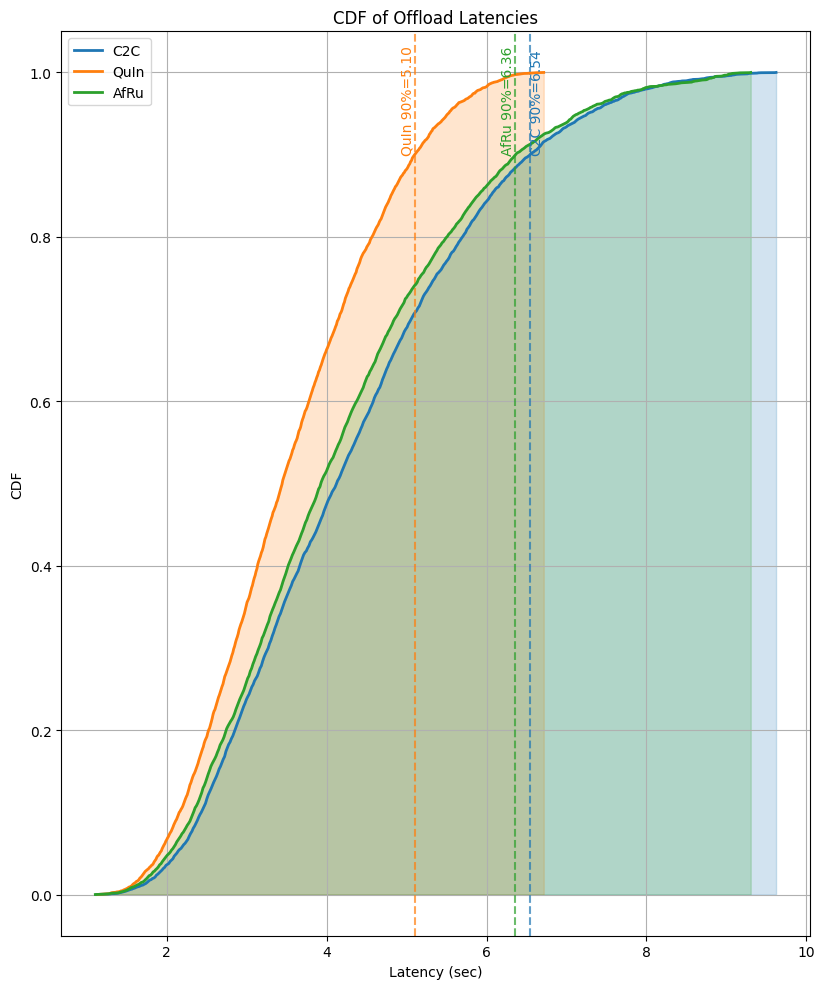
\includegraphics[width=0.7\textwidth]{CDF.pdf}
\caption{توزیع تجمعی تاخیر برای الگوریتم‌های شبیه‌سازی شده.}
\label{figure:CDF_plot}
\end{figure}
\vspace{0.5cm}

نمودار~\ref{figure:worst_plot} تاثیر افزایش بار در شبکه بر بیشترین تاخیر را بررسی می‌کند. بیشترین تاخیر ممکن در شبکه، نزدیک‌ترین زمان اجرای برنامه به مهلت وظیفه است که بیش از سایر وظایف عدم تجاوز از مهلت را به مخاطره می‌اندازد. به همین جهت در تابع هدف از عبارتی استفاده کردیم تا بیشینه تاخیر را کمینه کند. آنچنان که در نمودار دیده می‌شود، محور عمودی بیشینه تاخیر بر حسب ثانیه است. نقاط نمودار مرتبط با میانگین این مقادیر در اجراهای مختلف است. فضای ابری پیرامون نقاط نیز انحراف از این مقادیر را نشان می‌دهد. برای الگوریتم \lr{\tt{AfRu}}محدودیت در چیدمان، هرچند موجب جلوگیری از هم‌مکانی برنامه‌هایی می‌شود که بیشترین رقابت را دارند، اما با قوانین سخت‌گیرانه در نهایت موجب محدودیت در تنوع چینش می‌شود در حالی که شاید برخی تاخیرها هرچند زیاد، در شرایط موجود قابل پذیرش باشد و از مهلت وظیفه تجاوز نکند. محدودیت در چینش نهایتا ممکن است باعث بوجود آمدن ترکیب ناهمگون دیگری شود که تدبیر قانون هم‌پیوندی برای پیش‌بینی تداخل آن ناکافی بوده است. در نهایت مشخص است که تاخیر بیشینه در الگوریتم پیشنهادی ما کاهش محسسوسی یافته است.

\vspace{0.5cm}
\begin{figure}[h]
\centering
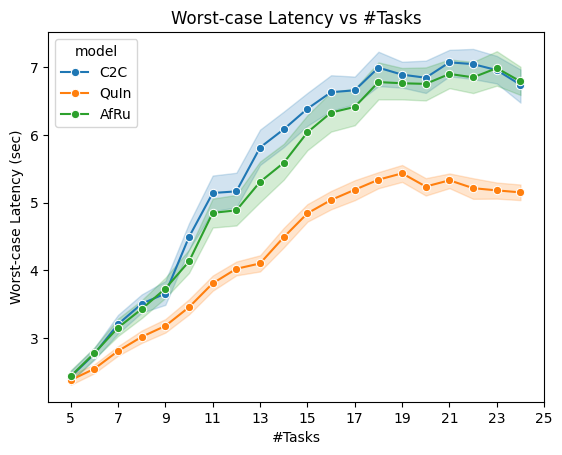
\includegraphics[width=0.7\textwidth]{worst.pdf}
\caption{بیشینه تاخیر با افزایش تعداد تقاضا.}
\label{figure:worst_plot}
\end{figure}
\vspace{0.5cm}

نمودار ~\ref{figure:colocate_plot} تاثیر تعداد برنامه‌های هم‌مکان بر تداخل را بررسی می‌کند. محور افقی نمودار تعداد برنامه‌های هم‌مکان در یک سرور را نشان می‌دهد. هر ستون نمودار چارک بندی شده به نوعی توزیع تاخیر را نشان می‌دهد. همچنین توسط الگوریتم رسم کننده نقاط پرت به صورت دایره‌هایی توخالی مشخص شده است. عملکرد بهینه الگوریتم ما نسبت به رقبا، حاصل جانمایی هوشمند کارنتینرها بر اساس رفتار تداخلی آن‌هاست. زیرا الگوریتم ارائه شده در این پژوهش توانایی تخمین کمی تداخل را دارد و همچون قانون هم‌پیوندی صرفا به اقدامی پیشگیرانه اکتفا نمی‌کند. در بار زیاد که موجب جانمایی حداکثری کانتینرها در یک سرور شده است، میانه تاخیرهای الگوریتم ارائه شده در این پژوهش بیش از ۲۰ درصد بهبود عملکرد را نشان می‌دهد. هم‌چنین با بررسی دم نمودارها در شرایط بار زیاد واضح است حتی دم اجرای الگوریتم پیشنهادی ما کمتر از میانه الگوریتم‌های رقیب است و با حالتی که ۵ کانتینر هم‌مکان شوند قابل مقایسه است.

\vspace{0.5cm}
\begin{figure}[h]
\centering
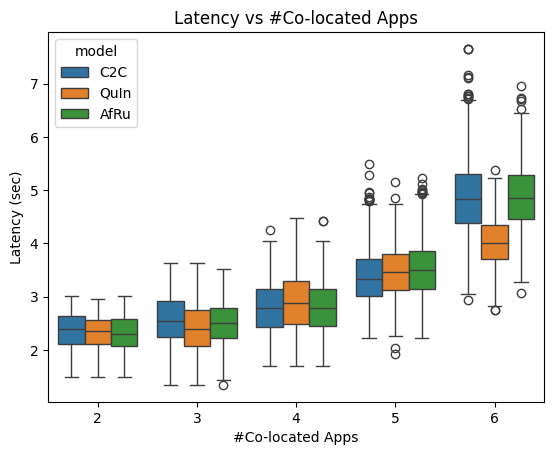
\includegraphics[width=0.7\textwidth]{colocate.pdf}
\caption{توزیع تاخیر اجرای برنامه‌ها با افزایش تعداد برنامه‌های هم‌مکان.}
\label{figure:colocate_plot}
\end{figure}
\vspace{0.5cm}

در نهایت برای ارزیابی مصالحه بین استفاده حداکثری از منابع پردازشی سرورها و جلوگیری از تداخل، نمودار~\ref{figure:util_plot} رسم شده است. این نمودار با تغییر بار توسط افزایش تعداد وظایف شبکه رسم شده است. در محور افقی نیز تعداد وظایف نمایش داده شده است. همانطور که در نمودار مشاهده می‌شود، الگوریتم پیشنهادی ما علاقه کمتری به استفاده حداکثری از منابع پردازشی سرورها را ارائه کرده است. زیرا الگوریتم ما ترجیح به تداخل کمتر می‌دهد. این رفتار می‌تواند با بررسی توان مصرفی برق متعادل شود. اما همین رویکرد باعث نرخ حذف پایینتر، حاشیه امن بیشتر تا مهلت تاخیر و توزیع تاخیر با مشخصات آماری کمتر شده است. پس از اشباع ظرفیت، همه منابع پردازشی مورد مصرف قرار گرفتند.

\vspace{0.5cm}
\begin{figure}[h]
\centering
\includegraphics[width=0.7\textwidth]{util.pdf}
\caption{میزان بهره‌برداری از توان پردازشی با افزایش تعداد تقاضا.}
\label{figure:util_plot}
\end{figure}
\vspace{0.5cm}

\section{نتیجه‌گیری}
این پژوهش، به مسئله‌ی برون‌سپاری وظایف در محیط‌های \lr{\tt{MEC}} پرداخته است. جایی که منابع محدود سرور، تأخیرهای ارتباطی و تداخل سخت‌افزاری میان برنامه‌ها به طور مشترک بر اجرا تأثیر می‌گذارند. در حالی که مطالعات پیشین عمدتاً بر تأخیر ارتباطی یا قواعد ساده‌ی هم‌پیوندی برای کاهش تداخل تمرکز داشته‌اند، این رویکردها در ارائه‌ی مدلی کمّی برای بازنمایی رقابت میان چندین برنامه هم‌مکان ناکام مانده‌اند. 

برای غلبه بر این محدودیت، ما یک مدل تداخل کمّی پیشنهاد دادیم که فراتر از تعاملات دوتایی برنامه‌ها عمل می‌کند و افت عملکرد ناشی از هم‌مکانی چندین برنامه را در نظر می‌گیرد. این مدل بر پایه‌ی آمارهای سطح پایین به‌دست‌آمده از اجرای تنهای برنامه ارائه شد، سپس به عوامل قابل‌تفسیرِ مرتبط با بهره‌وری منابع تبدیل گردید و با بهره‌گیری از برنامه‌های محک، تخمین مدل تداخل انجام گرفت. این مدل در قالب یک فرمول‌بندی مساله بهینه‌سازی ادغام شد. رویکرد پیشنهادی امکان تصمیم‌گیری‌های برون‌سپاری آگاه به تداخل فراهم کرد؛ به‌گونه‌ای که میان تأخیر ارتباطی، محدودیت‌های پردازش محلی و افت عملکرد ناشی از رقابت سخت‌افزاری تعادل برقرار گردد.

از طریق شبیه‌سازی و ارزیابی در برابر دو رویکرد رقیب از جمله قواعد هم‌پیوندی، نتایج نشان داد که رویکرد پیشنهادی ما عملکرد بهتری از جهت نرخ حذف درخواست‌ها به دلیل اتمام مهلت تاخیر، بهبود حاشیه امن بین زمان اجرا تا مهلت وظیفه و کاهش سایر مولفه‌های آماری تاخیر را دارد. 

در جمع‌بندی، این پژوهش یک مدل نوین و کمّیِ آگاه به تداخل ارائه می‌دهد که در برون‌سپاری وظایف \lr{\tt{MEC}} عملکرد چشمگیری دارد. با پر کردن شکاف میان دیدگاه‌های سنجش تداخل کیفی در تخصیص منابع و سنجش تداخل کمی بین تنها دو برنامه، این کار بنیانی کامل‌تر برای طراحی سامانه‌های \lr{\tt{MEC}} کارا و قابل‌اعتماد فراهم می‌کند؛ سامانه‌هایی که قادر به پشتیبانی از برنامه‌های حساس به تأخیر در محیط‌های مشترک و دارای محدودیت منابع هستند.